%%%% Proceedings format for most of ACM conferences (with the exceptions listed below) and all ICPS volumes.
\documentclass[sigconf]{acmart}
%%%% As of March 2017, [siggraph] is no longer used. Please use sigconf (above) for SIGGRAPH conferences.

%%%% Proceedings format for SIGPLAN conferences 
% \documentclass[sigplan, anonymous, review]{acmart}

%%%% Proceedings format for SIGCHI conferences
% \documentclass[sigchi, review]{acmart}

%%%% To use the SIGCHI extended abstract template, please visit
% https://www.overleaf.com/read/zzzfqvkmrfzn


\usepackage{booktabs} % For formal tables
\usepackage{placeins}
\usepackage{graphicx}
\usepackage{subcaption}

% Copyright
%\setcopyright{none}
%\setcopyright{acmcopyright}
%\setcopyright{acmlicensed}
%%%%\setcopyright{rightsretained}
%\setcopyright{usgov}
%\setcopyright{usgovmixed}
%\setcopyright{cagov}
%\setcopyright{cagovmixed}


\usepackage{algorithm}


% Graph Libraries TIKZ START
\usepackage{tikz}
\usepackage{verbatim}
\usetikzlibrary{arrows,shapes}

% Declare layers
\pgfdeclarelayer{background}
\pgfsetlayers{background,main}

\tikzstyle{vertex}=[circle,fill=black!25,minimum size=20pt,inner sep=0pt]
\tikzstyle{selected vertex} = [vertex, fill=red!24]
\tikzstyle{edge} = [draw,thick,-]
\tikzstyle{weight} = [font=\small]
\tikzstyle{selected edge} = [draw,line width=5pt,-,red!50]
\tikzstyle{ignored edge} = [draw,line width=5pt,-,black!20]
% Graph Libraries TIKZ END


\begin{document}
\title{CapsGraph : Algorithmic Framework for Learning Diverse Spatial Knowledge Graphs using Capsule Networks}

\def\matthias#1{{\sc \textcolor{green}{Matthias says: }}{\marrow\sf \textcolor{red}{#1}}}
\def\pavlos#1{{\sc \textcolor{blue}{Pavlos says: }}{\marrow\sf \textcolor{red}{#1}}}
\def\hardik#1{{\sc \textcolor{red}{Hardik says: }}{\marrow\sf \textcolor{red}{#1}}}


\author{Hardik Patel}
\affiliation{%
  \institution{Dep. of Computational and Data Sciences}
  \institution{George Mason University}
  \city{Fairfax}
  \state{Virginia}
}
\email{hpatel12@gmu.edu}


% \author{Pavlos Paraskevopoulos}
% \affiliation{%
%   \institution{Dep. of Computational and Data Sciences, Datalab}
%   \institution{George Mason University}
%   \city{Fairfax}
%   \state{Virginia}
% }
% \email{pparaske@gmu.edu}

\author{Matthias Renz}
\affiliation{%
  \institution{Professor, Data Science}
  \institution{University of Kiel}
  \city{Kiel}
  \state{Germany}
}
\email{mr@informatik.uni-kiel.de}


\begin{abstract}
CapsGraph framework applies successful deep-learning models on multi-dimensional spatial knowledge graphs. In this process, we extract semantic knowledge graph from text documents, transform graph into vectors using node prioritization. We generate Heterogeneous Information Network from node attributes and edge information of knowledge graph. We generate embedding model based on CapsNet for Neural Network where each capsule is group of neurons whose activity vector is instantiated with vectors of HIN. We apply this methodology for similarity search of document from collection of inordinate number of documents.
\end{abstract}



% \keywords{data fusion, Heterogeneous Networks, knowledge enrichment, Twitter, OSM, Trajectories}


\maketitle

\section{Introduction and motivation}
\label{sec:introduction}
The domain of knowledge graph generated from text data is variable based on data, unlike graph generated from Social Networks where domain is fixed. Here, we capture their structure, node attributes and edge attributes for learning which makes this a data-driven approach to generate network embedding. Furthermore, knowledge extraction from text is a complex problem that introduces noise. By using embedding that is a higher level abstraction provides estimation that is similar to cognitive inference. 

Capsule networks (referred to as CapsNets), which are proposed as an alternative counterpart to convolutional neural networks (CNNs). Here we introduce a powerful new approach for learning generative models over knowledge graphs using CapsNet, which can capture their structure with node and edge attributes. Our approach uses CapsNet to express probabilistic dependencies among a graph's nodes and edges, and can, in principle, learn distributions over any arbitrary graph. In a series of experiments our results show that once trained, our models are efficient for document similarity and classification.
% \section{Motivation}
Data sets generated from social networks, crowd sourcing, IoT devices and predictive analysis consists of large number of interconnected, multi-typed components that is modelled as heterogeneous information networks (HINs). Traditional methods of analyzing HINs over such huge amount of data sets makes it impractical to use. Furthermore, social networks and crowd sourced databases could polluted with machine generated data that makes traditional graph traversal methods for data mining and analysis unusable unless additional work is performed to sanitize input data. Additionally, traditional methods to generate Knowledge Base from HINs requires computations in the order of magnitude of nodes and edges. Similarly, analysis images and text generated from these platforms is also a challenge that has been successfully overcome by using neural network based machine learning methods on massively distributed systems with high speed memory and processors. Capsule networks is one of deep learning method that has produced promising results by overcoming short falls of CNN. These advancements in deep learning and success of CapsNet is our motivation behind creating algorithm for applying CapsNet architecture for knowledge base of diverse nature with geo-spatial information.
\section{Related Work}
In past decades information network analysis has become a hot research topic in data mining and information retrieval fields \cite{shi2017survey}. There are various research areas that focus on learning heterogeneous information networks that include clustering \cite{huang2016meta}, classification \cite{kong2012meta}, link prediction \cite{zhang2017link}, similarity \cite{sun2011pathsim}, etc. Although, these algorithmic methods are well defined on complex heterogeneous meta-structures, it require algorithmic processing of complete graph. Alternatively, information retrieval algorithms from HINs proposes random walk models to evaluate relevance of different-typed objects that requires defined data structure and node types. Furthermore, these traditional approaches does not work with expanded node links because of generic node labels without creating direct links.

In recent years automatic feature learning algorithms are at the forefront of machine learning research and deep learning has been successfully adopted in many applications such as speech recognition and image classification. Furthermore, graph clustering methods based on deep neural network \cite{tian2014learning} have produced promising results. While CNNs are very successful in various supervised learning applications, it falls behind in AI related applications. Deep reinforcement learning (RL) models are major improvement over traditional deep learning in terms of capacity, training time and sample size \cite{zambaldi2018relational}. Reinforcement learning is efficiently utilized in graph structures \cite{liang2017deep}. CapsNet resolves issues with CNNs by applying dynamic routing between capsules. Our novel graph embedding model is based on CapsNet for unsupervised learning on knowledge graphs generated from heterogeneous data sources because of localized characteristics of small independent graph structures.
\section{Background}
We provide brief introduction to capsule networks and convolutional networks in deep learning in context of graph theory.

\paragraph{Covolutional Neural Networks}
Convolutional Neural Networks (ConvNets or CNNs) are a category of Neural Networks that have proven very effective in areas such as image recognition and classification.
\begin{figure}[!htbp]
  \centering
  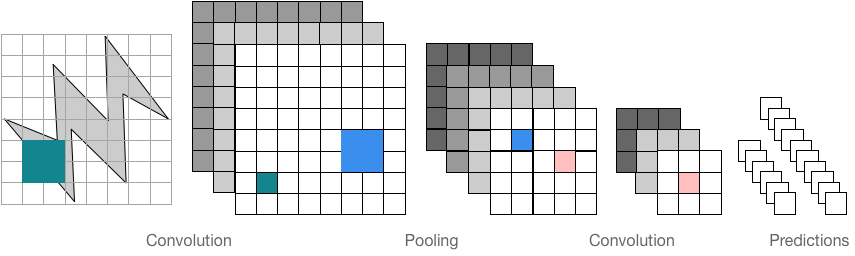
\includegraphics[width=\linewidth,height=\textheight,keepaspectratio]{images/CNN.png}
  \caption{CNN}
  \label{cnn}
\end{figure}
\FloatBarrier
Basic building blocks of Convolutional Neural Network are Convolution, Non Linearity (ReLU), Pooling or and Classification. When CNNs are used to classify images, a grid is move over each image with a particular step size. The receptive field reads the feature values for each channel in specific spatial order. The spatial order uniquely determines nodes of each receptive field and the way these nodes are mapped to a vector space representation. The values read from two pixels using two locations of receptive fields are assigned to the same relative position if and only if the pixels' structural roles are identical.

\paragraph{Capsule Network}
Convolutional neural networks work very well in various deep learning tasks but it has fundamental drawback. Simple example is rotated image \ref{k}. Orientational and relative spatial relationships between components are less important in CNN sicne higher-level features combine lower level features as a weighted sum that is sum of activations of preceding layers multiplied by weights. In this process relationshipe between simpler features are lost that make up higher level feature. To solve this problem CNNs use max pooling or successive layers to reduce spacial size of the data flowing through the network. Although, max pooling works well, it looses spatial information on features.
Capsule is a group of neurons whose activity represents the instantiation parameters of entities. The length of the activity vector represents the probability that the entity exists and its orientation to represent the instantiation parameters. In Caps net allows to keep relative relationship between objects which is represented as multi dimentional matrix.

\begin{figure}[!htbp]
  \centering
  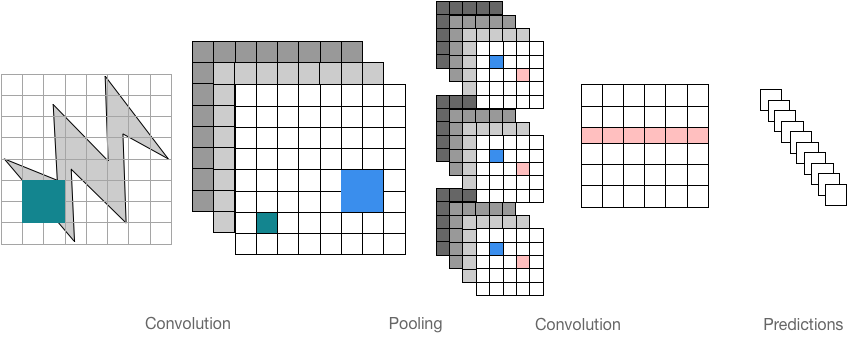
\includegraphics[width=\linewidth,height=\textheight,keepaspectratio]{images/CapsNet.png}
  \caption{Capsule Network Architecture}
  \label{k}
\end{figure}
\FloatBarrier

\section{Proposed Model}
In this section, we first define our approach to generate knowledge graph from document text and graph translation before generating graph embedding for CapsNet.
\subsection{Knowledge Graph from Text}
To build knowledge graph from document text requires extract entities and relations. This approach is ideal for fixed domain such as social networks and HIN from social networks. When domain is not fixed, for large number of documents, it becomes impractical to gather such training data that can do entity extraction. As defined earlier, we are creating multi dimensional HIN that is higher level abstraction of domain and relationship between nodes. Hence, we use pre-trained model BERT\cite{devlin2018bert}.

BERT model comes pre-trained on large corpus.  

\subsection{Graph Translation}
Our goal is to derive $ S= \{ s_i_j \}$ that is similarity matrix of directed graph $ G $, where  $ s_i_j (i, j=1, 2, ... n) $ is the similarity score between node $i$ and $j$. $G=(E,V,W)$ where $V=\{ v_1,...,_n \} $ is the set of vertices and  $E  \subseteq V \times V$ set of edges. Let $ n $ be the number of vertices and $ m $ the number of edges. $G$ is directed graph with $e_i_j=1$ for edge $i \to j$ and $e_i_j=-1$ for edge $j \to i$. We allow, each edge $(i,j)$ to have corresponding weight $w_i_j \in W$. Furthermore, each vertex $v_i$ has feature vector $l_i$.
CapsGraph has three steps: 1. Generate static sub-graphs with defined vertex ordering, 2. Create convolution layers using local substructure, 3. Learn graph structures using capsule filters.

\subsection{Capsule Network for Graph}

\begin{figure}[!htbp]
  \centering
  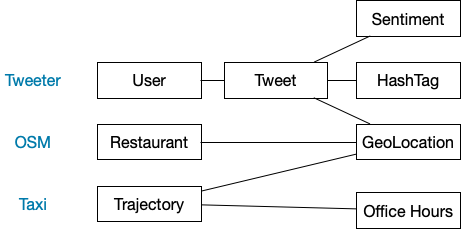
\includegraphics[width=\linewidth,height=\textheight,keepaspectratio]{images/Sample_Data}
  \caption{Original Dataset}
  \label{sample_data}
\end{figure}

\subsection{Graph Translation Algorithm}
In order to create neighbourhood matrix that represents vertex in consistent order we used sorting algorithm based on in-degree and out-degree of nodes. First, part is to create sub-graph that is represents context of node entities. In order to generate sub-graph, we first visit each neighboring node and compare depth from starting node to connected edges of visiting node which becomes terminating factor for sub-graph.

% \subsection{Graph Convolutional Layer}
% \subsection{Capsule Layer}
% \begin{figure}
% \begin{tikzpicture}[scale=1.8, auto,swap]
%     % Draw a 7,11 network
%     % First we draw the vertices
%     \foreach \pos/\name in {{(0,2)/a}, {(2,1)/b}, {(4,1)/c},
%                             {(0,0)/d}, {(3,0)/e}, {(2,-1)/f}, {(4,-1)/g}}
%         \node[vertex] (\name) at \pos {$\name$};
%     % Connect vertices with edges and draw weights
%     \foreach \source/ \dest /\weight in {b/a/7, c/b/8,d/a/5,d/b/9,
%                                          e/b/7, e/c/5,e/d/15,
%                                          f/d/6,f/e/8,
%                                          g/e/9,g/f/11}
%         \path[edge] (\source) -- node[weight] {$\weight$} (\dest);
%     % Start animating the vertex and edge selection. 
%     \foreach \vertex / \fr in {d/1,a/2,f/3,b/4,e/5,c/6,g/7}
%         \path<\fr-> node[selected vertex] at (\vertex) {$\vertex$};
%     % For convenience we use a background layer to highlight edges
%     % This way we don't have to worry about the highlighting covering
%     % weight labels. 
%     \begin{pgfonlayer}{background}
%         \pause
%         \foreach \source / \dest in {d/a,d/f,a/b,b/e,e/c,e/g}
%             \path<+->[selected edge] (\source.center) -- (\dest.center);
%         \foreach \source / \dest / \fr in {d/b/4,d/e/5,e/f/5,b/c/6,f/g/7}
%             \path<\fr->[ignored edge] (\source.center) -- (\dest.center);
%     \end{pgfonlayer}
% \end{tikzpicture}
% \end{figure}

\FloatBarrier
% \subsection{Training}

\begin{figure}[!htbp]
  \centering
  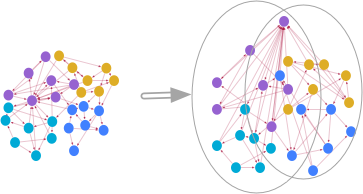
\includegraphics[width=\linewidth,height=\textheight,keepaspectratio]{images/graph_normalization}
  \caption{Graph Representation Model}
  \label{graph_model}
\end{figure}
% \section{Experiments} 
In this section we look at two experiments of using CapsGraph for semi-supervised deep learning of knowledge graphs. The first experiment uses generated knowledge graph from patents text obtained from USPTO (United States Patent and Trademark Office) for text analysis and second experiment uses labelled data from FDA (Food and Drug Administration) for link analysis. Both data-sets are publicly available and code is available on Github.
\subsection{Semi-supervised learning for text data}
This dataset is patents data files that has various fields and lot of unstructured text. Goal is to implement MLT (More Like This) feature to search similar patents to a given text of patent summary. The problem we are trying to solve is to find documents ("patents") similar to a given document and not a specific document. One document may have multiple parts and one of the parts may contain similarity to another whole document. Such "partial match" should be given higher priority. We will create embedding from documents such that related documents are close to each other in embedding space. We create document-document graph such that they share edges. The relationship between documents is coming from graph (HIN). Sentence query of word query will not work here since it will not capture graph data. We can start First step is information extraction from unstructured text to create knowledge graph.

\subsubsection{Knowledge Graph from Text} 
Natural Language Processing (NLP) techniques have advanced a lot in last decade. Various language models have been proposed for estimation of word representations in vector space, such as Word2Vec\cite{mikolov2013efficient} and GloVe\cite{Pennington2014GloveGV}. Here we use ELMo (Embeddings from Language Models)\cite{Peters_2018}. First we extract named entities from text and create a linked graph of specific meta structure by extracting entities and relations in specific domain. Next step is to extract information about the entities by finding relation between the extracted entities and object. At document (patent) level it is less important to preserve each entity relation respective to the document, hence, it is possible use probability apply filter using attention model to keep only relevant information at document level. To focus only on relevant parts of the document, we create trigram embedding to create vectors for each trigram and send it to attention layer to determine weights. 
\par Our goal is to encode nodes

\subsubsection{CapsGraph embedding from knowledge graph}
Our data is composed of RDF Triples as described in GeoTeGra\cite{patel2018geotegra}. First, we generate 3xN matrix for each triple where each column vector represents embedding of triple element. We create multiple layers for each subgraph. In one document we can create subgraph of relevant sentences or paragraphs. Entities resulted from ELMo can be one layer. In addition to NER, we also processed the document using NLP where we find relationship between entities. There relationship can be "mentions" of entity type and create another layer.

\subsubsection{Document similarity evaluation}
In the task of finding similar document for a given document, the results are calculated based on ranking of scores produces by sum of score functions on triples. To evaluate the results we evaluate similarity between each triple of source document and top 5 resulting document.

% \section{Conclusion}
\bibliographystyle{ACM-Reference-Format}
\bibliography{capsgraph,text-vectors}

\end{document}